\section{Experimento BRDF Cook-Torrance}\label{sec:cook-torrance}

Este experimento é baseada no modelo microfacetado que descreve o comportamento de reflexão de superfícies metálicas descrito no trabalho de Cook-Torrance \cite{cook1982reflectance}. As equações e parametros escolhidos que descrevem esse modelo estão em \autoref{fig-cook-torrance-eqlang-latex}. O código fonte em \texttt{EquationLang} para o compilador está em \autoref{cod-cook-torrance-eqlang}. O código GLSL está dividido em duas partes, parte 1 está no \autoref{cod-cook-torrance-glsl-pt-1} e a segunda parte está em \autoref{cod-cook-torrance-glsl-pt-2}. A renderização dos objetos 3D usando essa BRDF se encontra em \autoref{fig-cook-torrance-eqlang}. Usamos plot logaritmo para gerar os plots 3D e polar presentes na \autoref{fig-cook-torrance-plots}.

%%%%%%%%%%%%%%%%%%%%%%%%%%%%%%%%%%%%%%%%%%%%%%%%%
\subsection{Representação em documento \LaTeX{}}
%%%%%%%%%%%%%%%%%%%%%%%%%%%%%%%%%%%%%%%%%%%%%%%%%
\begin{figure}[H]
    \caption{\label{fig-cook-torrance-eqlang-latex} \small Equações da BRDF do experimento cook-torrance em documento \LaTeX{}.}
    \begin{center}
        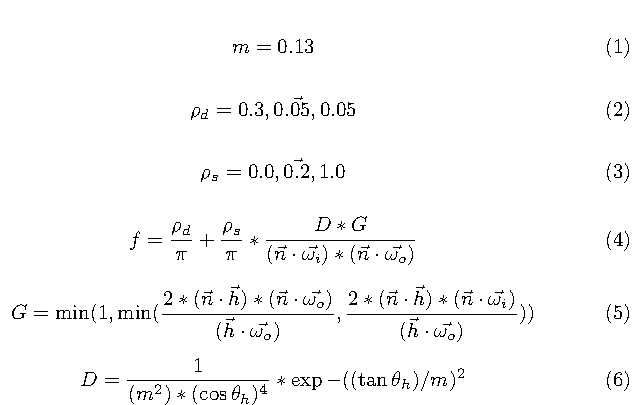
\includegraphics[scale=0.92]{./Imagens/brdfs/cook-torrance.pdf}
    \end{center}
\end{figure}

%%%%%%%%%%%%%%%%%%%%%%%%%%%%%%%%%%%%%%%%%%%%%%%%%
\subsection{Visualização do Resultado}
%%%%%%%%%%%%%%%%%%%%%%%%%%%%%%%%%%%%%%%%%%%%%%%%%
\begin{figure}[H]
    \caption{\small{\textit{Plots} da BRDF deste experimentos.}}\label{fig-cook-torrance-plots}
\minipage{0.48\textwidth}
    \vspace{42px}
  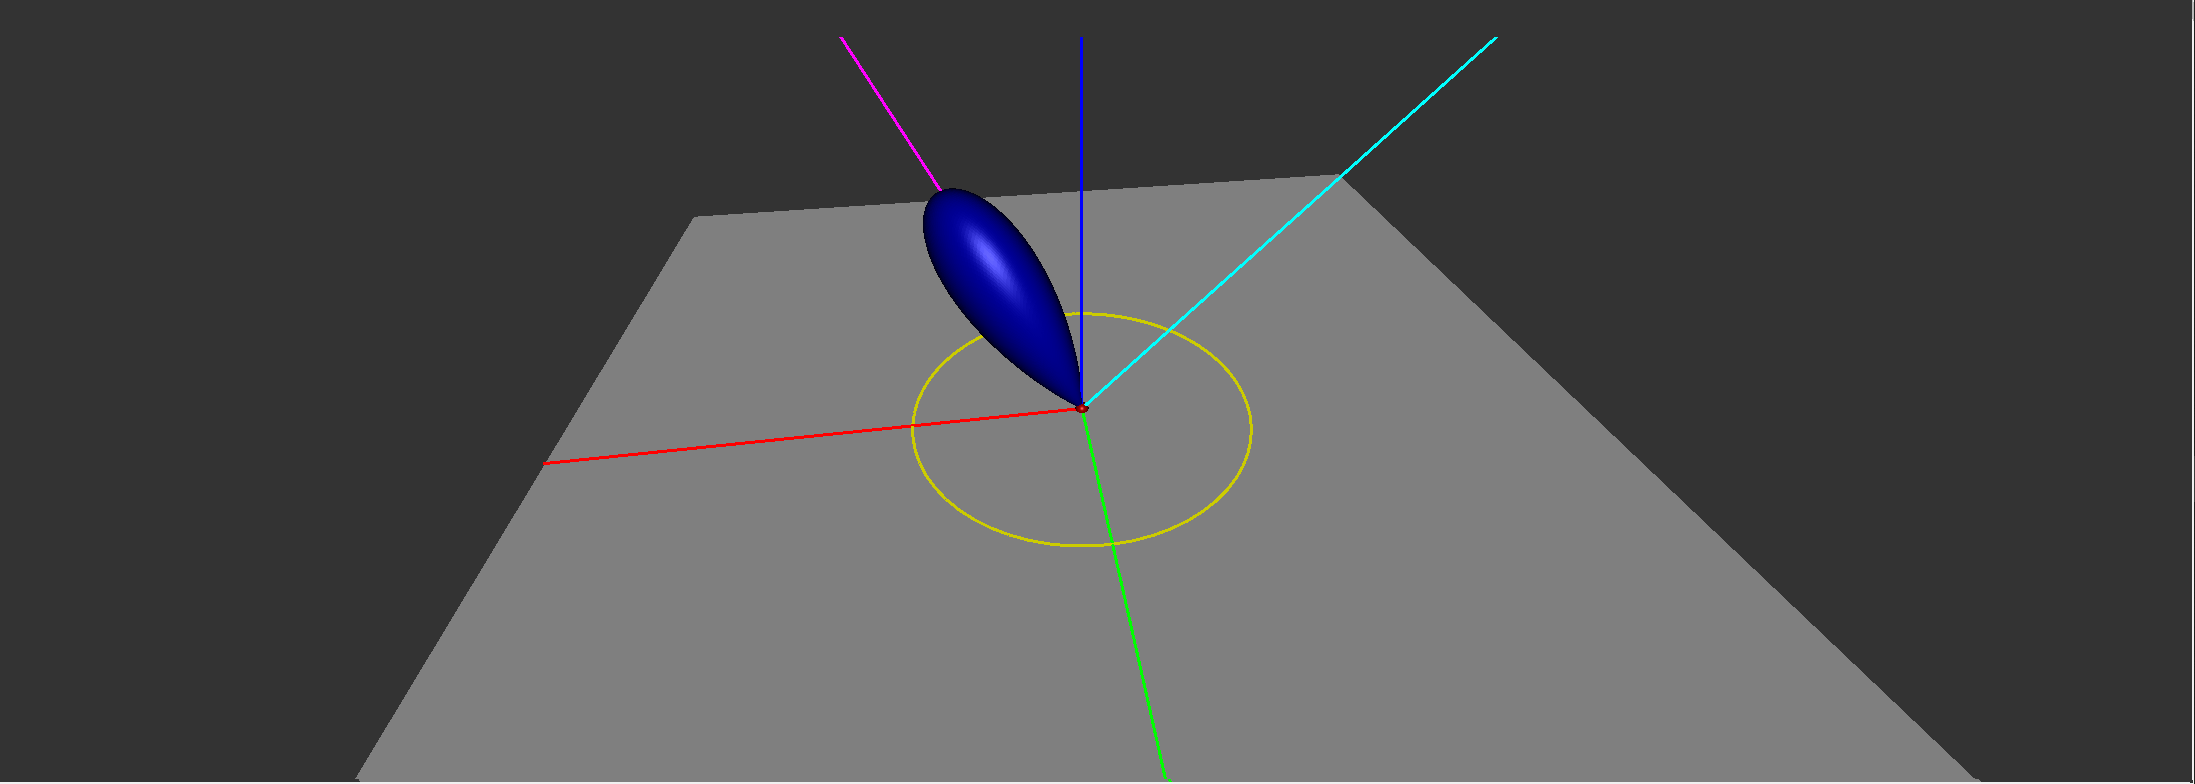
\includegraphics[width=\linewidth]{./Imagens/brdfs/cook-torrance-3D-plot}
    % \vspace{0.1px}
    \legend{ \small (a) 3D \textit{plot}}
\endminipage\hfill
\minipage{0.48\textwidth}
  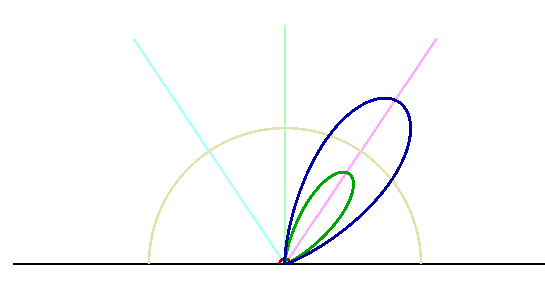
\includegraphics[width=\linewidth]{./Imagens/brdfs/cook-torrance-polar-plot-log.png}
    \legend{ \small (b) \textit{Polar plot}}
\endminipage\hfill
\end{figure}

\begin{figure}[H]
    \caption{\small{Objetos 3D renderizados por este experimento}}\label{fig-cook-torrance-eqlang}
\minipage{0.32\textwidth}
  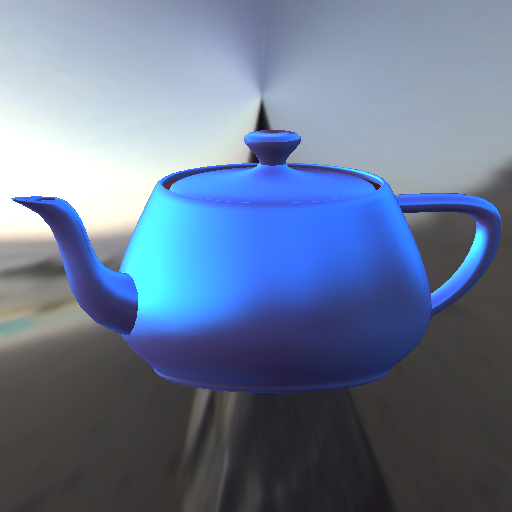
\includegraphics[width=\linewidth]{./Imagens/brdfs/cook-torrance-teapot.png}
    \legend{ \small (a) \textit{Teapot}}
\endminipage\hfill
\minipage{0.32\textwidth}
  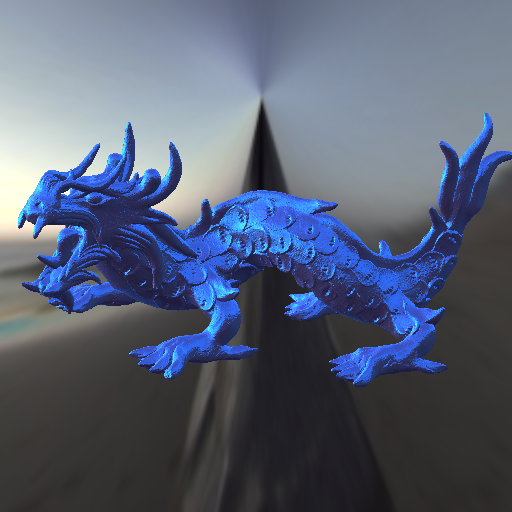
\includegraphics[width=\linewidth]{./Imagens/brdfs/cook-torrance-dragon.png}
    \legend{ \small (b) Dragão de Stanford}
\endminipage\hfill
\minipage{0.32\textwidth}%
  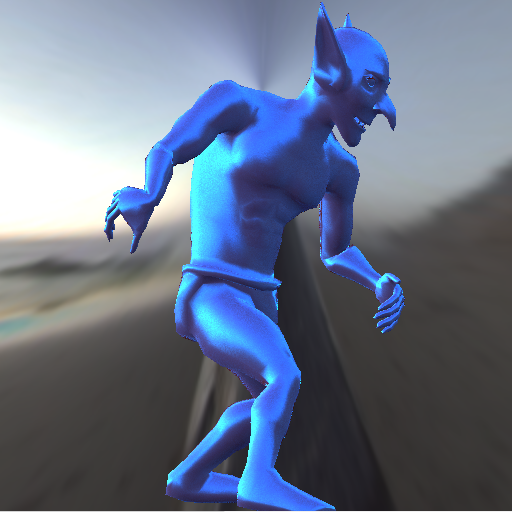
\includegraphics[width=\linewidth]{./Imagens/brdfs/cook-torrance-goblin.png}
    \legend{ \small (c) Goblin}
\endminipage
\end{figure}

%%%%%%%%%%%%%%%%%%%%%%%%%%%%%%%%%%%%%%%%%%%%%%%%%
\subsection{Código GLSL Gerado}
%%%%%%%%%%%%%%%%%%%%%%%%%%%%%%%%%%%%%%%%%%%%%%%%%
\begin{codigo}[H]
    \caption{\small Saida do compilador, código GLSL da BRDF deste experimento (parte 1). }
    \label{cod-cook-torrance-glsl-pt-1}
\begin{lstlisting}[language=C, inputencoding=utf8]
analytic ::begin parameters
#[type][name][min val][max val][default val]
::end parameters
::begin shader
//////////// START OF BUILTINS DECLARTION ////////////
vec3 var_0_vec_h;
vec3 var_3_vec_n;
float var_10_theta_h;
float var_11_theta_d;
float var_1_pi;
float var_2_epsilon;
vec3 var_4_vec_omega_i;
float var_5_theta_i;
float var_6_phi_i;
vec3 var_7_vec_omega_o;
float var_8_theta_o;
float var_9_phi_o;
//////////// END OF BUILTINS DECLARTION ////////////
//////////// START OF USER DECLARED ////////////
float var_12_G;
vec3 var_13_rho_s;
float var_14_m;
float var_15_D;
vec3 var_16_rho_d;
vec3 var_17_f;
//////////// END OF USER DECLARED ////////////
//////////// START FUNCTIONS DECLARATIONS ////////////
//////////// END FUNCTIONS DECLARATIONS ////////////
\end{lstlisting}
\end{codigo}

\begin{codigo}[H]
    \caption{\small Saida do compilador, código GLSL da BRDF deste experimento  (parte 2). }
    \label{cod-cook-torrance-glsl-pt-2}
\begin{lstlisting}[language=C, inputencoding=utf8]
vec3 BRDF(vec3 L, vec3 V, vec3 N, vec3 X, vec3 Y) {

  //////////// START OF BUILTINS INITIALIZATION ////////////
  var_0_vec_h = normalize(L + V);
  var_3_vec_n = normalize(N);
  var_1_pi = 3.141592653589793;
  var_2_epsilon = 1.192092896e-07;
  var_4_vec_omega_i = L;
  var_5_theta_i = atan(var_4_vec_omega_i.y, var_4_vec_omega_i.x);
  var_6_phi_i = atan(sqrt(var_4_vec_omega_i.y * var_4_vec_omega_i.y +
                          var_4_vec_omega_i.x * var_4_vec_omega_i.x),
                     var_4_vec_omega_i.z);
  var_7_vec_omega_o = V;
  var_8_theta_o = atan(var_7_vec_omega_o.y, var_7_vec_omega_o.x);
  var_9_phi_o = atan(sqrt(var_7_vec_omega_o.y * var_7_vec_omega_o.y +
                          var_7_vec_omega_o.x * var_7_vec_omega_o.x),
                     var_7_vec_omega_o.z);
  var_10_theta_h = acos(dot(var_0_vec_h, N));
  var_11_theta_d = acos(dot(var_0_vec_h, var_4_vec_omega_i));
  //////////// END OF BUILTINS INITIALIZATION ////////////

  var_12_G = min(1.0, min((((2.0 * (dot(var_3_vec_n, var_0_vec_h))) *
                            (dot(var_3_vec_n, var_7_vec_omega_o))) /
                           (dot(var_0_vec_h, var_7_vec_omega_o))),
                          (((2.0 * (dot(var_3_vec_n, var_0_vec_h))) *
                            (dot(var_3_vec_n, var_4_vec_omega_i))) /
                           (dot(var_0_vec_h, var_7_vec_omega_o)))));
  var_13_rho_s = vec3(0.0, 0.2, 1.0);
  var_14_m = 0.13;
  var_15_D = ((1.0 / ((pow(var_14_m, 2.0)) * pow((cos(var_10_theta_h)), 4.0))) *
              exp((-pow((((tan(var_10_theta_h)) / var_14_m)), 2.0))));
  var_16_rho_d = vec3(0.3, 0.05, 0.05);
  var_17_f =
      ((var_16_rho_d / var_1_pi) +
       ((var_13_rho_s / var_1_pi) *
        ((var_15_D * var_12_G) / ((dot(var_3_vec_n, var_4_vec_omega_i)) *
                                  (dot(var_3_vec_n, var_7_vec_omega_o))))));

  return vec3(var_17_f);
}
\end{lstlisting}
\end{codigo}

%%%%%%%%%%%%%%%%%%%%%%%%%%%%%%%%%%%%%%%%%%%%%%%%%
\subsection{Código Fonte em \texttt{EquationLang}}
%%%%%%%%%%%%%%%%%%%%%%%%%%%%%%%%%%%%%%%%%%%%%%%%%
\begin{codigo}[H]
    \caption{\small Código fonte da BRDF deste experimento.}
    \label{cod-cook-torrance-eqlang}
\begin{lstlisting}[language=tex, frame=none, inputencoding=utf8]
\begin{equation}
m = 0.13
\end{equation}

\begin{equation}
    \rho_{d} = \vec{0.3,0.05,0.05}
\end{equation}

\begin{equation}
    \rho_{s} = \vec{0.0,0.2,1.0}
\end{equation}

\begin{equation}
f = \frac{\rho_{d}}{\pi} +
\frac{\rho_{s}}{\pi} *
\frac{D*G}{({\vec{n}}\cdot{\vec{\omega_{i}}}) *
({\vec{n}}\cdot{\vec{\omega_{o}}})}
\end{equation}

\begin{equation}
G = \min(1,\min(
\frac{2 *
({\vec{n}}\cdot{\vec{h}}) *
({\vec{n}}\cdot{\vec{\omega_{o}}})
}
{({\vec{h}}\cdot{\vec{\omega_{o}}})},
\frac{2 *
({\vec{n}}\cdot{\vec{h}}) *
({\vec{n}}\cdot{\vec{\omega_{i}}})
}
{({\vec{h}}\cdot{\vec{\omega_{o}}})}
))
\end{equation}

\begin{equation}
D = \frac{1}
{(m^{2}) * (\cos{\theta_{h}})^{4}} *
\exp{-((\tan{\theta_{h}})/m)^{2}}
\end{equation}
\end{lstlisting}
\end{codigo}
